%%%%%%%%%%%%%%%%%%%%%%%%%%%%%%%%%%%%%%%%%%%%%%%%%%%%%%%%%%%%%%%%%%%%%%%%
% Slide options
%%%%%%%%%%%%%%%%%%%%%%%%%%%%%%%%%%%%%%%%%%%%%%%%%%%%%%%%%%%%%%%%%%%%%%%%

% Option 1: Slides with solutions

\documentclass[slidestop,compress,mathserif]{beamer}
\usepackage{booktabs}
\newcommand{\soln}[1]{\textit{#1}}
\newcommand{\solnGr}[1]{#1}

% Option 2: Handouts without solutions

%\documentclass[11pt,containsverbatim,handout]{beamer}
%\usepackage{pgfpages}
%\pgfpagesuselayout{4 on 1}[letterpaper,landscape,border shrink=5mm]
%\newcommand{\soln}[1]{ }
%\newcommand{\solnGr}{ }

%%%%%%%%%%%%%%%%%%%%%%%%%%%%%%%%%%%%%%%%%%%%%%%%%%%%%%%%%%%%%%%%%%%%%%%%
% Style
%%%%%%%%%%%%%%%%%%%%%%%%%%%%%%%%%%%%%%%%%%%%%%%%%%%%%%%%%%%%%%%%%%%%%%%%
%%%%%%%%%%%%%%%%%%%%%%%%%%%%%%%%%%%%%%%%%%%%%%%%%%%%%%%%%%%%%%%%%%%%%%%%
% MA213/214 shared slide style
%
% "Calm & Cool" palette + content-type callout boxes.
% Overhauled (2026) from the original OpenIntro/metropolis style:
%   - all OpenIntro visual branding removed (logo, grid, colors)
%   - a low-key cool palette (see colors below)
%   - tcolorbox callout boxes so students recognize content types
% See common/README.md for the command cheat-sheet.
%%%%%%%%%%%%%%%%%%%%%%%%%%%%%%%%%%%%%%%%%%%%%%%%%%%%%%%%%%%%%%%%%%%%%%%%

\usetheme{metropolis}

%%%%%%%%%%%%%%%%
% Packages
%%%%%%%%%%%%%%%%

\usepackage{geometry}
\usepackage{graphicx}
\usepackage{amssymb}
\usepackage{epstopdf}
\usepackage{amsmath}  	% this permits text in eqnarray among other benefits
\usepackage{url}		% produces hyperlinks
\usepackage{hyperref}	% allows for color usage in tables
\usepackage[english]{babel}
\usepackage[latin1]{inputenc}
\usepackage{colortbl}	% allows for color usage in tables
\usepackage{multirow}	% allows for rows that span multiple rows in tables
\usepackage{color}		% this package has a variety of color options
\usepackage{pgf}
\usepackage{calc}
\usepackage{ulem}
\usepackage{multicol}
\usepackage{textcomp}
\usepackage{txfonts}
\usepackage{listings}
\usepackage{tikz}
\usepackage{array}
\usepackage{wasysym}
\usepackage{fancyvrb}
\usepackage{etoolbox}             % \ifstrempty for optional box subtitles
\usepackage[most]{tcolorbox}      % content-type callout boxes
\tcbuselibrary{listings}          % R-code block (\begin{rblock})
\usepackage{fontawesome5}         % box icons

%%%%%%%%%%%%%%%%
% Remove navigation symbols
%%%%%%%%%%%%%%%%

\setbeamertemplate{navigation symbols}{}

%%%%%%%%%%%%%%%%
% "Calm & Cool" palette
%%%%%%%%%%%%%%%%

% chrome / structure / body
\definecolor{ccSlate}{HTML}{2E3742}   % frametitle bar, structure, section pages (deep neutral slate)
\definecolor{ccInk}{HTML}{2B2B2B}     % body text
\definecolor{ccWash}{HTML}{FCF8F1}    % gentle warm title-slide background wash (complements the cool blues)

% example (blue)
\definecolor{ccBlue}{HTML}{2F6690}
\definecolor{ccBlueBg}{HTML}{EAF1F7}
% interactive activity / discussion (green)
\definecolor{ccGreen}{HTML}{4E8A6B}
\definecolor{ccGreenBg}{HTML}{E9F3EC}
% solution (purple)
\definecolor{ccPurple}{HTML}{6F5499}
\definecolor{ccPurpleBg}{HTML}{EFEAF6}
% worksheet / focused work (terracotta)
\definecolor{ccTerra}{HTML}{C2693E}
\definecolor{ccTerraBg}{HTML}{FAEDE4}
% formula / definition (neutral slate)
\definecolor{ccGray}{HTML}{5C6B7A}
\definecolor{ccGrayBg}{HTML}{EEF1F4}
% caution / common pitfall (brick red)
\definecolor{ccRed}{HTML}{B23A48}
\definecolor{ccRedBg}{HTML}{FAEAEC}
% key idea / takeaway (muted gold)
\definecolor{ccGold}{HTML}{9C7A28}
\definecolor{ccGoldBg}{HTML}{F7F1DF}
% learning goals / lesson outcomes (teal)
\definecolor{ccTeal}{HTML}{2C6E6B}
\definecolor{ccTealBg}{HTML}{E6F0EF}
% learning objectives (indigo)
\definecolor{ccIndigo}{HTML}{45507A}
\definecolor{ccIndigoBg}{HTML}{ECEEF4}
% R code / output (gray)
\definecolor{ccCode}{HTML}{5F5E5A}
\definecolor{ccCodeBg}{HTML}{F4F5F6}

% neutral grays kept from the original style
\definecolor{gray}{rgb}{0.5, 0.5, 0.5}
\definecolor{darkGray}{rgb}{0.3, 0.3, 0.3}
\definecolor{darkerGray}{rgb}{0.2, 0.2, 0.2}

% Backwards-compatible aliases: old OpenIntro color names now point at the
% new palette, so existing \textcolor{oiB}{...}, \hl{...}, etc. keep working.
\colorlet{oiB}{ccBlue}
\colorlet{oiG}{ccGreen}
\colorlet{hlblue}{ccBlue}
\colorlet{rubineRed}{ccRed}
\colorlet{irishGreen}{ccGreen}
\colorlet{lightGreen}{ccGreen}

%%%%%%%%%%%%%%%%
% Restyle metropolis with the Calm & Cool chrome
%%%%%%%%%%%%%%%%

\metroset{block=fill}

\setbeamercolor{normal text}{fg=ccInk, bg=white}
\setbeamercolor{structure}{fg=ccSlate}
\setbeamercolor{alerted text}{fg=ccBlue}
\setbeamercolor{example text}{fg=ccGreen}
\setbeamercolor{frametitle}{bg=ccSlate, fg=white}
\setbeamercolor{progress bar}{fg=ccBlue}
\setbeamercolor{title separator}{fg=ccBlue}
\setbeamercolor{title}{fg=ccSlate}
\setbeamercolor{subtitle}{fg=ccBlue}
\setbeamercolor{author}{fg=ccInk}
\setbeamercolor{institute}{fg=ccGray}
\setbeamercolor{date}{fg=ccGray}
\setbeamercolor{section title}{fg=ccSlate}
\setbeamercolor{standout}{fg=white, bg=ccSlate}

% Section pages sit on the same warm wash as the title slide. We keep
% metropolis's section-title styling and just paint a full-page ccWash
% background behind it (needs >=2 pdflatex passes for the current-page node).
\setbeamertemplate{section page}{%
  \begin{tikzpicture}[remember picture, overlay]
    \fill[ccWash] (current page.south west) rectangle (current page.north east);
  \end{tikzpicture}%
  \centering
  \begin{minipage}{22em}
    \raggedright
    \usebeamercolor[fg]{section title}%
    \usebeamerfont{section title}%
    \insertsectionhead\\[-1ex]
    \usebeamertemplate*{progress bar in section page}%
    \par
  \end{minipage}\par
  \vspace{\baselineskip}
}

%%%%%%%%%%%%%%%%
% Custom inline text commands (recolored to the palette)
%%%%%%%%%%%%%%%%

% degree
\newcommand{\degree}{\ensuremath{^\circ}}

% cite
\newcommand{\ct}[1]{
\vfill
{\tiny #1}}

\newcommand{\NamedNote}[2]{
\rule{2.5cm}{0.25pt} \\ \textit{\footnotesize{\textcolor{rubineRed}{#1:} \textcolor{darkerGray}{#2}}}}

% Note
\newcommand{\Note}[1]{
\rule{2.5cm}{0.25pt} \\ \textit{\footnotesize{\textcolor{rubineRed}{Note:} \textcolor{darkerGray}{#1}}}}

% Remember
\newcommand{\Remember}[1]{\textit{\scriptsize{\textcolor{ccTerra}{Remember:} #1}}}

% expected counts
\newcommand{\ex}[1]{\textit{\textcolor{ccBlue}{#1}}}

% red
\newcommand{\red}[1]{\textit{\textcolor{rubineRed}{#1}}}

% pink
\newcommand{\pink}[1]{\textit{\textcolor{rubineRed!90!white!50}{#1}}}

% green
\newcommand{\green}[1]{\textit{\textcolor{irishGreen}{#1}}}

% orange
\newcommand{\orange}[1]{\textit{\textcolor{ccTerra}{#1}}}

% links: webURL, webLink, appLink
\newcommand{\webURL}[1]{\urlstyle{same}{ \textit{\textcolor{darkGray}{\url{#1}}}}}
\newcommand{\webLink}[2]{\href{#1}{\textcolor{darkGray}{{#2}}}}
\newcommand{\appLink}[2]{\href{#1}{\textcolor{white}{{#2}}}}

% mail
\newcommand{\mail}[1]{\href{mailto:#1}{\textit{\textcolor{darkGray}{#1}}}}

% highlighting: hl, hlGr, mathhl
\newcommand{\hl}[1]{\textit{\textcolor{hlblue}{#1}}}
\newcommand{\hlGr}[1]{\textit{\textcolor{lightGreen}{#1}}}
\newcommand{\mathhl}[1]{\textcolor{hlblue}{\ensuremath{#1}}}

%%%%%%%%%%%%%%%%
% Structural helpers (unchanged from the original)
%%%%%%%%%%%%%%%%

% two col: two columns
\newenvironment{twocol}[4]{
\begin{columns}[c]
\column{#1\textwidth}
#3
\column{#2\textwidth}
#4
\end{columns}
}

% slot (for probability calculations)
\newenvironment{slot}[2]{
\begin{array}{c}
\underline{#1} \\
#2
\end{array}
}

% pr: left and right parentheses
\newcommand{\pr}[1]{
\left( #1 \right)
}

% cancel
\newcommand{\cancel}[1]{%
    \tikz[baseline=(tocancel.base)]{
        \node[inner sep=0pt,outer sep=0pt] (tocancel) {#1};
        \draw[red, line width=0.5mm] (tocancel.south west) -- (tocancel.north east);
    }%
}

% removepagenumbers
\newcommand{\removepagenumbers}{%
  \setbeamertemplate{footline}{}
}

% change margin
\newenvironment{changemargin}[2]{%
\begin{list}{}{%
\setlength{\topsep}{0pt}%
\setlength{\leftmargin}{#1}%
\setlength{\rightmargin}{#2}%
\setlength{\listparindent}{\parindent}%
\setlength{\itemindent}{\parindent}%
\setlength{\parsep}{\parskip}%
}%
\item}{\end{list}}

% footnote
\long\def\symbolfootnote[#1]#2{\begingroup%
\def\thefootnote{\fnsymbol{footnote}}\footnote[#1]{#2}\endgroup}

% commands from the book
\newenvironment{data}[1]{\texttt{#1}}{}
\newenvironment{var}[1]{\texttt{#1}}{}
\newenvironment{resp}[1]{\texttt{#1}}{}

%%%%%%%%%%%%%%%%
% Content-type callout boxes (tcolorbox)
%
% Each type has a colored title strip (icon + label) over a light fill.
% Color = content type; the label + icon reinforce it (so the cue does
% not rely on color alone).
%%%%%%%%%%%%%%%%

\tcbset{
  cccallout/.style 2 args={
    enhanced, breakable=false,
    colback=#2, colframe=#1, colbacktitle=#1, coltitle=white,
    fonttitle=\bfseries\footnotesize,
    boxrule=0.6pt, arc=2.5pt, outer arc=2.5pt,
    left=5pt, right=5pt, top=3pt, bottom=3pt, boxsep=2pt,
    toptitle=2pt, bottomtitle=2pt, lefttitle=5pt,
    before skip=5pt, after skip=5pt,
  },
}

% One-off / collection of examples (blue): \workedexample[subtitle]{body}.
% (Named \workedexample, not \example, because beamer defines \example.)
\newtcolorbox{examplebox}[1][]{cccallout={ccBlue}{ccBlueBg},
  title={\faIcon{lightbulb}~~Example\ifstrempty{#1}{}{ \textmd{---}\ #1}}}
\newcommand{\workedexample}[2][]{\begin{examplebox}[#1]#2\end{examplebox}}

% Running-example header (blue): \examplehead{name} at the top of each frame of a
% multi-slide running example. A one-off or a collection of examples uses the
% \workedexample box above instead.
\newcommand{\examplehead}[1]{%
  \vspace{-0.4em}\par\noindent\tcbox[on line, colback=ccBlue, colframe=ccBlue, coltext=white,
    boxrule=0pt, arc=2pt, left=5pt, right=5pt, top=1pt, bottom=1pt,
    box align=base, nobeforeafter]{\footnotesize\bfseries\faIcon{lightbulb}\,Running example}%
  \ifstrempty{#1}{}{\enspace{\footnotesize\bfseries\textcolor{ccBlue}{#1}}}%
  \par\nobreak\vspace{-0.6em}{\color{ccBlue}\rule{\linewidth}{0.7pt}}\par\nobreak\vspace{-0.8em}}

% Interactive activity (green): \activity[subtitle]{body}
\newtcolorbox{activitybox}[1][]{cccallout={ccGreen}{ccGreenBg},
  title={\faIcon{users}~~Activity\ifstrempty{#1}{}{ #1}}}
\newcommand{\activity}[2][]{\begin{activitybox}[#1]#2\end{activitybox}}

% Discussion question (green): \dq{body}
\newtcolorbox{dqbox}{cccallout={ccGreen}{ccGreenBg}, title={\faIcon{comments}~~Discussion}}
\newcommand{\dq}[1]{\begin{dqbox}#1\end{dqbox}}

% Solution (purple): \solnbox{body}. Gated by the per-deck \soln toggle, so it
% shows in the instructor build and vanishes from the student handout build.
% (Named \solnbox, not \solution, because beamer already defines \solution.)
\newtcolorbox{solutionbox}{cccallout={ccPurple}{ccPurpleBg}, title={\faIcon{key}~~Solution}}
\newcommand{\solnbox}[1]{\soln{\begin{solutionbox}#1\end{solutionbox}}}

% Worksheet / focused work (terracotta): \worksheet[subtitle]{body}
\newtcolorbox{worksheetbox}[1][]{cccallout={ccTerra}{ccTerraBg},
  title={\faIcon{pencil-alt}~~Worksheet\ifstrempty{#1}{}{ #1}}}
\newcommand{\worksheet}[2][]{\begin{worksheetbox}[#1]#2\end{worksheetbox}}

% Formula / definition (neutral slate). Supports both real usages found in the
% decks: \formula{title}{body} and the bare \formula{body} (title defaults to
% "Formula"). The second group is an optional brace argument.
\newtcolorbox{formulabox}[1][Formula]{cccallout={ccGray}{ccGrayBg},
  title={\faIcon{square-root-alt}~~#1}}
\NewDocumentCommand{\formula}{m g}{%
  \IfNoValueTF{#2}%
    {\begin{formulabox}#1\end{formulabox}}%
    {\begin{formulabox}[#1]#2\end{formulabox}}}

% Common pitfall / caution (brick red): \caution[subtitle]{body}
\newtcolorbox{cautionbox}[1][]{cccallout={ccRed}{ccRedBg},
  title={\faIcon{exclamation-triangle}~~Caution\ifstrempty{#1}{}{ #1}}}
\newcommand{\caution}[2][]{\begin{cautionbox}[#1]#2\end{cautionbox}}

% Key idea / takeaway (muted gold): \keyidea[subtitle]{body}
\newtcolorbox{keyideabox}[1][]{cccallout={ccGold}{ccGoldBg},
  title={\faIcon{star}~~Key idea\ifstrempty{#1}{}{ #1}}}
\newcommand{\keyidea}[2][]{\begin{keyideabox}[#1]#2\end{keyideabox}}

% Learning goals / lesson outcomes (teal): \goals{body}. Sits under the short
% LO headings on the objectives slide; body is the "you should be able to" list.
\newtcolorbox{goalsbox}{cccallout={ccTeal}{ccTealBg}, fontupper=\footnotesize,
  top=1pt, bottom=2pt, boxsep=1pt, before skip=3pt,
  title={\faIcon{bullseye}~~By the end of today, you should be able to\ldots}}
\newcommand{\goals}[1]{\begin{goalsbox}#1\end{goalsbox}}

% Learning objectives (indigo): \objectives{body} -- the formal LO headings,
% shown alongside \goals on the objectives slide.
\newtcolorbox{objectivesbox}{cccallout={ccIndigo}{ccIndigoBg}, fontupper=\small,
  top=1pt, bottom=2pt, boxsep=1pt, before skip=3pt,
  title={\faIcon{clipboard-list}~~Learning objectives}}
\newcommand{\objectives}[1]{\begin{objectivesbox}#1\end{objectivesbox}}

% Defaults for a bare \begin{lstlisting}. Without these it inherits the listings
% package defaults: 11pt type, fixed-width columns (which spaces code out as
% "a g e _ f i t"), and no line breaking, so a long line silently runs off the
% right edge of the slide. A deck that passes its own basicstyle still wins.
% Layout only -- syntax coloring is left to the \begin{rblock} environment.
\lstset{
  basicstyle=\ttfamily\footnotesize, columns=fullflexible,
  breaklines=true, breakindent=1.5em, showstringspaces=false,
  numbers=none, frame=none}

% R code / output (gray): \begin{rblock}[subtitle] ... \end{rblock}
% NOTE: a frame containing an rblock must be declared \begin{frame}[fragile].
\lstdefinestyle{ccR}{
  language=R, basicstyle=\ttfamily\footnotesize, columns=fullflexible,
  breaklines=true, showstringspaces=false, numbers=none, frame=none,
  keywordstyle=\color{ccBlue}, commentstyle=\color{ccGreen!75!black},
  stringstyle=\color{ccTerra}}
\newtcblisting{rblock}[1][]{cccallout={ccCode}{ccCodeBg},
  title={\faIcon{terminal}~~R\ifstrempty{#1}{}{ #1}},
  listing only, listing style=ccR}

% --- Legacy boxes (kept so existing decks compile) ---

% app: application exercise -> alias of activity
\newcommand{\app}[1]{\activity{#1}}

% pq: practice question (green, interactive family)
\newtcolorbox{pqbox}{cccallout={ccGreen}{ccGreenBg}, title={\faIcon{list-ol}~~Practice}}
\newcommand{\pq}[1]{\begin{pqbox}#1\end{pqbox}}

% solnMult: solutions for multiple-choice practice questions (uses \soln toggle)
\newcommand{\solnMult}[1]{
\item[] \vspace{-0.59cm}
\only<1>{\item #1}
\soln{\only<2->{\item \orange{#1}}}
}

%%%%%%%%%%%%%%%%
% De-branded title frame + attribution
%%%%%%%%%%%%%%%%

% Eyebrow line on the title slide; a deck may \renewcommand this.
\newcommand{\coursetag}{MA214: Applied Statistics}

% Attribution: all slides released under CC BY-SA, crediting both the
% instructor (later material) and OpenIntro (basis of the earlier material).
\newcommand{\courseattribution}{%
  Slides by Jonathan H.~Huggins, building on materials from OpenIntro's
  \emph{Introduction to Modern Statistics} (Mine \c{C}etinkaya-Rundel et al.).
  Released under the
  \webLink{http://creativecommons.org/licenses/by-sa/3.0/us/}{CC BY-SA license}.
  Some images included under fair use (educational purposes).}

% \maketitleframe: de-branded title slide (no logo, no grid). Uses the deck's
% \title, \subtitle, and \coursetag.
\newcommand{\maketitleframe}{%
  \addtocounter{framenumber}{-1}%
  {\removepagenumbers
  \setbeamercolor{background canvas}{bg=ccWash}%
  \begin{frame}[plain]
    \vspace*{2.6em}
    {\color{ccSlate}\rule{\textwidth}{2.5pt}}\par\vspace{1.5em}
    {\usebeamerfont{date}\scshape\color{ccGray}\coursetag}\par\vspace{0.55em}
    {\usebeamerfont{title}\color{ccSlate}\inserttitle\par}
    \vspace{0.45em}{\color{ccBlue}\rule{3em}{2.5pt}}\par\vspace{0.7em}
    {\usebeamerfont{subtitle}\color{ccBlue}\insertsubtitle\par}
    \vfill
    {\color{ccGray!55}\rule{\textwidth}{0.4pt}}\par\vspace{0.45em}
    {\tiny\color{ccGray}\courseattribution\par}
    \vspace*{0.4em}
  \end{frame}}}

%%%%%%%%%%%%%%%%
% Graphics
%%%%%%%%%%%%%%%%

\DeclareGraphicsRule{.tif}{png}{.png}{`convert #1 `dirname #1`/`basename #1 .tif`.png}

\graphicspath{ {../../common/} }


%%%%%%%%%%%%%%%%%%%%%%%%%%%%%%%%%%%%%%%%%%%%%%%%%%%%%%%%%%%%%%%%%%%%%%%%
% Preamble
%%%%%%%%%%%%%%%%%%%%%%%%%%%%%%%%%%%%%%%%%%%%%%%%%%%%%%%%%%%%%%%%%%%%%%%%

\title[Lecture 4]{Lecture 4: Using Regression Models}
\subtitle{Module 1: Modeling and Linear Regression}
\author{Introduction to Modern Statistics, 2nd Edition}
\institute{$\:$ \\ {\footnotesize  Based on slides developed by Mine \c{C}etinkaya-Rundel of OpenIntro.  \\
The slides may be copied, edited, and/or shared via the \webLink{http://creativecommons.org/licenses/by-sa/3.0/us/}{CC BY-SA license.} \\
Some images may be included under fair use guidelines (educational purposes).}}
\date{}

%%%%%%%%%%%%%%%%%%%%%%%%%%%%%%%%%%%%%%%%%%%%%%%%%%%%%%%%%%%%%%%%%%%%%%%%
% Begin document
%%%%%%%%%%%%%%%%%%%%%%%%%%%%%%%%%%%%%%%%%%%%%%%%%%%%%%%%%%%%%%%%%%%%%%%%

\begin{document}


%%%%%%%%%%%%%%%%%%%%%%%%%%%%%%%%%%%%%%%%%%%%%%%%%%%%%%%%%%%%%%%%%%%%%%%%
% Title page
%%%%%%%%%%%%%%%%%%%%%%%%%%%%%%%%%%%%%%%%%%%%%%%%%%%%%%%%%%%%%%%%%%%%%%%%

\maketitleframe

% !TEX root =  Lecture4.tex


%%%%%%%%%%%%%%%%%%%%%%%%%%%%%%%%%%%%
% Recap/Agenda 
%%%%%%%%%%%%%%%%%%%%%%%%%%%%%%%%%%%%
\begin{frame}
    \frametitle{Module 1: Modeling and Linear Regression}
        \begin{itemize}
    \item \hl{Previously:} linear regression model and least squares.
    \item \hl{This time:} using a fitted regression model.
      \begin{itemize}
      \item correlation and $R^2$
      \item prediction, residuals, and extrapolation
      \item a first look at categorical predictors (more in Lecture 5)
      \end{itemize}
    \item \hl{Reading:} IMS Chapter 7.3--7.4.
    \end{itemize}
\end{frame}


%%%%%%%%%%%%%%%%%%%%%%%%%%%%%%%%%%%%
% Learning objectives:
%%%%%%%%%%%%%%%%%%%%%%%%%%%%%%%%%%%%
\begin{frame}
    \frametitle{Lecture Objectives}
    \goals{%
    \begin{itemize}
    \item interpret the meaning and fit of a linear regression model in context;
    \item interpret $r$ and $R^2$ as measures of direction, strength, and explained variability;
    \item use a fitted regression line for prediction, and distinguish interpolation from extrapolation.
    \end{itemize}}
    \objectives{%
    \begin{itemize}
    \item \textbf{(M1, LO2)} Understanding and Applying Linear Regression Models
    \item \textbf{(M1, LO3)} Using Regression Models
    \item \textbf{(M1, LO4)} Model Selection and $R^{2}$ and Adjusted $R^{2}$
    \end{itemize}}
\end{frame}

    
%%%%%%%%%%%%%%%%%%%%%%%%%%%%%%%%%%%%%%%%%%%%%%%%%%%%%%%%%%%%%%%%%%%%%%%%
\section{Using $R^2$ and correlation}
%%%%%%%%%%%%%%%%%%%%%%%%%%%%%%%%%%%%%%%%%%%%%%%%%%%%%%%%%%%%%%%%%%%%%%%%
\subsection{What does a good linear fit mean?}
%%%%%%%%%%%%%%%%%%%%%%%%%%%%%%%%%%%%%%%%%%%%%%%%%%%%%%%%%%%%%%%%%%%%%%%%
\begin{frame}
\frametitle{From fitting a line to using a line}

Given a fitted line
$$
\widehat{y}=\widehat{\beta}_0+\widehat{\beta}_1 x,
$$
and variance estimate $\hat{\sigma}^{2}$, we want to use them to answer questions! 
\begin{enumerate}
\item How strong is the linear relationship?
\item What prediction does the model make?
\item Is the prediction reasonable for a particular value of $x$?
\end{enumerate}
\end{frame}
%%%%%%%%%%%%%%%%%%%%%%%%%%%%%%%%%%%%%%%%%%%%%%%%%%%%%%%%%%%%%%%%%%%%%%%%
\begin{frame}
\frametitle{A running example}

A fresh dataset: across the 50 states, model \emph{poverty rate} from \emph{high-school graduation rate}.
\[
\widehat{\text{poverty}}=64.78-0.62(\text{HS grad}).
\]
\begin{columns}[T]
\begin{column}{0.52\textwidth}
\begin{itemize}
\item Response: poverty rate (\%).
\item Predictor: HS graduation rate (\%).
\item Slope: each extra point of HS graduation lowers predicted poverty by 0.62 points.
\end{itemize}
\end{column}
\begin{column}{0.48\textwidth}
\begin{center}
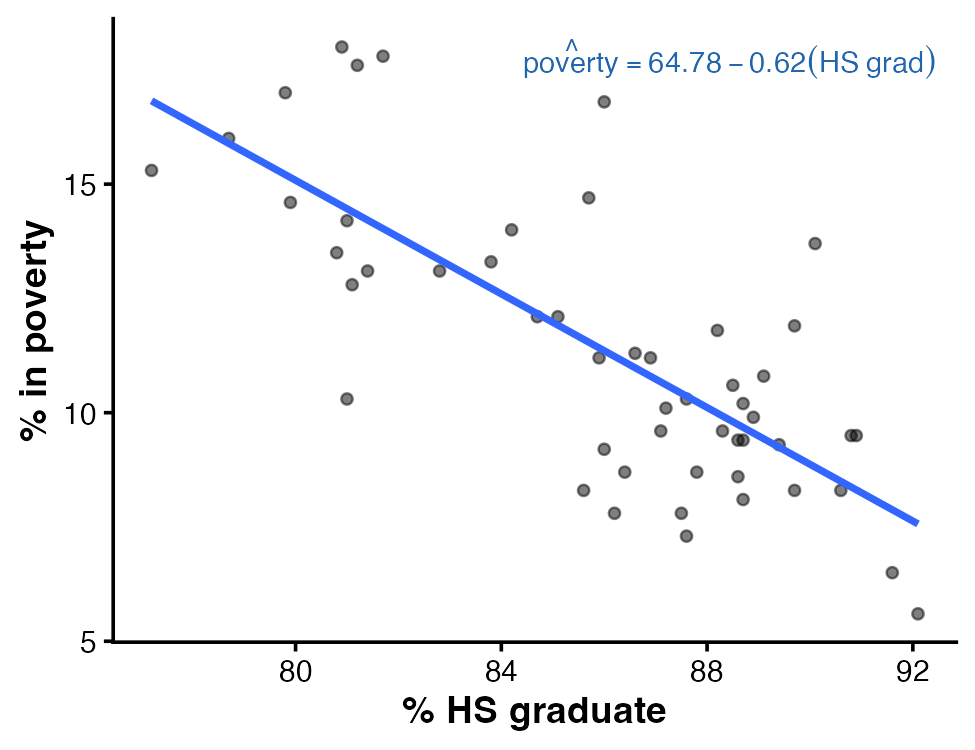
\includegraphics[width=0.9\textwidth]{figures/poverty-vs-hsgrad-line.png}
\end{center}
\end{column}
\end{columns}
\end{frame}
%%%%%%%%%%%%%%%%%%%%%%%%%%%%%%%%%%%%%%%%%%%%%%%%%%%%%%%%%%%%%%%%%%%%%%%%
\begin{frame}
\frametitle{Correlation coefficient}

The \textbf{correlation coefficient} $r$ measures the \textbf{direction} and \textbf{strength} of the \emph{linear} relationship between two numerical variables.

\formula{Correlation coefficient $r$}{%
$$
r=\frac{1}{n-1}\sum_{i=1}^n\left(\frac{x_i-\bar{x}}{s_x}\right)\left(\frac{y_i-\bar{y}}{s_y}\right)
$$
$-1\le r\le 1$: the \textbf{sign} gives the direction, and the \textbf{distance from 0} gives the strength of the linear trend.}

\end{frame}

%%%%%%%%%%%%%%%%%%%%%%%%%%%%%%%%%%%%%%%%%%%%%%%%%%%%%%%%%%%%%%%%%%%%%%%%

\begin{frame}
\frametitle{Interpreting $r$}

\begin{columns}[T]
\begin{column}{0.46\textwidth}
\begin{itemize}
\item $r$ near $1$: strong positive linear trend.
\item $r$ near $-1$: strong negative linear trend.
\item $r$ near $0$: weak \emph{linear} trend.
\end{itemize}

\vspace{0.4em}
Which panel has $r$ closest to $+1$? To $-1$? Near $0$?
\end{column}
\begin{column}{0.54\textwidth}
\begin{center}
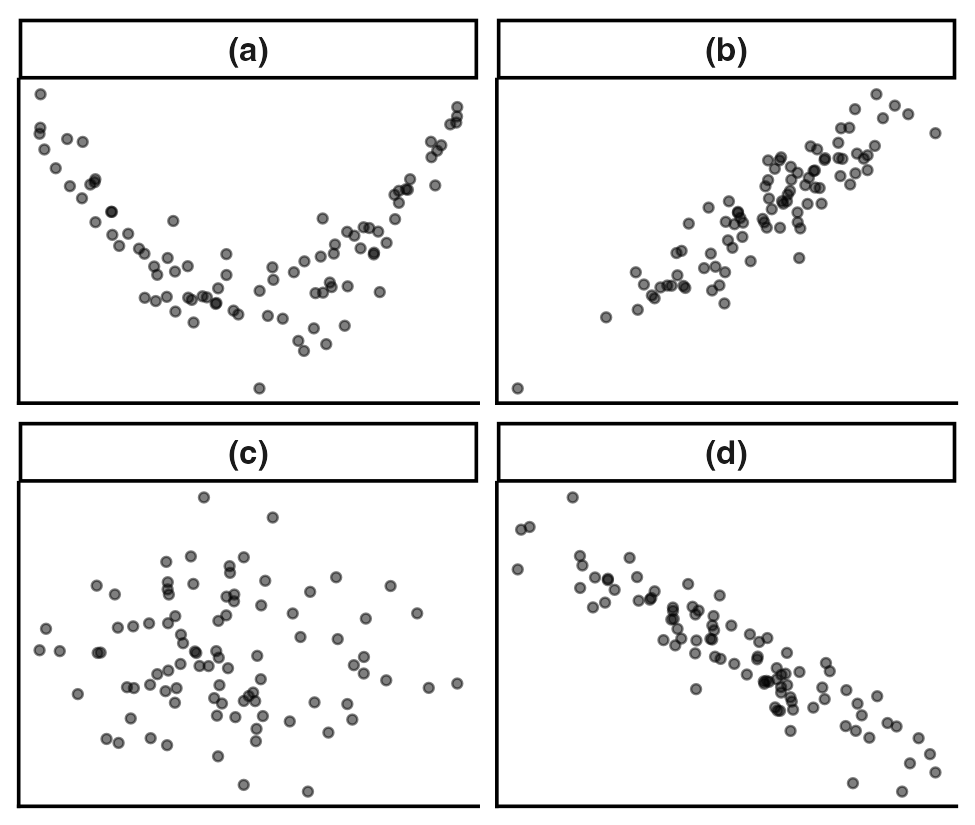
\includegraphics[width=0.95\textwidth]{figures/correlation-gallery.png}
\end{center}
\end{column}
\end{columns}
\end{frame}

%%%%%%%%%%%%%%%%%%%%%%%%%%%%%%%%%%%%%%%%%%%%%%%%%%%%%%%%%%%%%%%%%%%%%%%%
\begin{frame}
\frametitle{Coefficient of determination: $R^2$}
$$
R^2 = \frac{\text{variability explained by the model}}{\text{total variability in the response}}
$$
For simple regression, $R^2=r^2$, but we read $R^2$ off the model output rather than computing it from $r$.
\pause 
\begin{itemize}
\item Always between $0$ and $1$ (that is, $0\%$ to $100\%$).
\item Higher $R^2$ means the line accounts for more of the spread in $y$.
\item The remaining variability is due to other variables or natural randomness such as measurement error.
\end{itemize}
\pause
\keyidea[-- $R^2$]{$R^2$ is the \hl{percent of the variability in the response} that the linear model explains.}

\end{frame}
%%%%%%%%%%%%%%%%%%%%%%%%%%%%%%%%%%%%%%%%%%%%%%%%%%%%%%%%%%%%%%%%%%%%%%%%
\begin{frame}
\frametitle{What different $R^2$ values look like}
\begin{center}
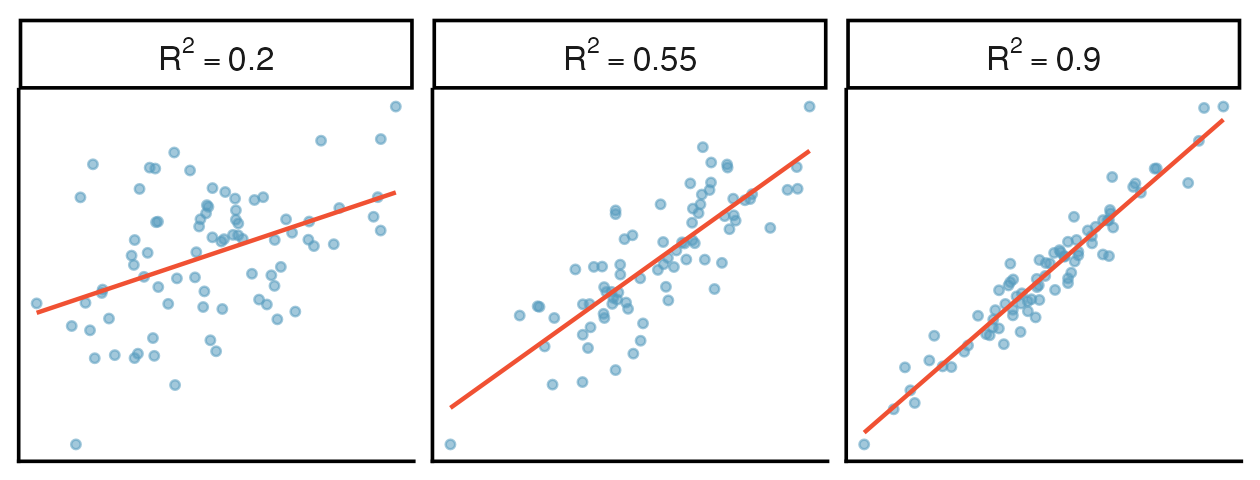
\includegraphics[width=\textwidth]{figures/r2-gallery.png}
\end{center}
For the poverty model, software reports $R^2=0.56$: about $56\%$ of the variability in poverty rate is explained by HS graduation rate.
\end{frame}
%%%%%%%%%%%%%%%%%%%%%%%%%%%%%%%%%%%%%%%%%%%%%%%%%%%%%%%%%%%%%%%%%%%%%%%%
\begin{frame}
\frametitle{Same $R^2$, very different data}
\begin{center}
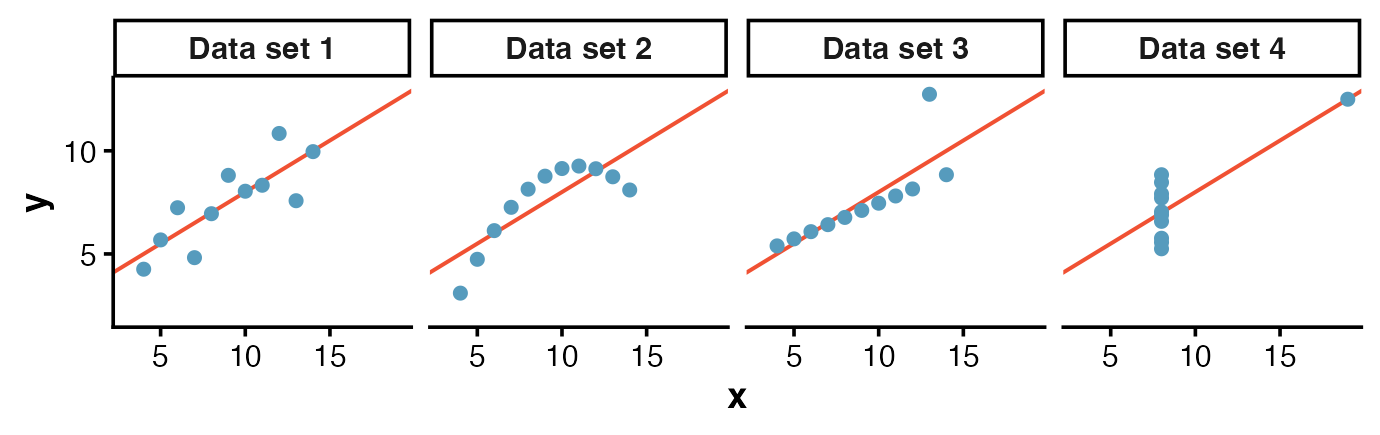
\includegraphics[width=\textwidth]{figures/anscombe.png}
\end{center}
All four data sets share the \hl{same fitted line} and the \hl{same $R^2=0.67$}, yet only the first is well described by a line.
\caution{$R^2$ alone does not tell you a line is appropriate. Always plot the data: a model you \emph{can} fit is not always one you \emph{should}.}
\end{frame}
%%%%%%%%%%%%%%%%%%%%%%%%%%%%%%%%%%%%%%%%%%%%%%%%%%%%%%%%%%%%%%%%%%%%%%%%
\begin{frame}
\frametitle{Common mistakes with $R^2$}

\activity[-- interpreting $R^2$]{%
Which statement is the best interpretation of $R^2=0.56$?
\begin{enumerate}
\item The model predicts 56\% of states exactly correctly.
\item HS graduation rate causes 56\% of the poverty rate.
\item 56\% of the variability in poverty rate is explained by the model.
\item The correlation is 0.56.
\end{enumerate}}

\pause
\solnbox{Correct: (3). $R^2$ describes explained variability, not exact prediction accuracy or causation.}

\end{frame}
%%%%%%%%%%%%%%%%%%%%%%%%%%%%%%%%%%%%%%%%%%%%%%%%%%%%%%%%%%%%%%%%%%%%%%%%
\begin{frame}
\frametitle{Activity: comparing simple regression models}

\activity[-- which model explains more?]{%
Three candidate models for predicting a state's poverty rate:
\begin{center}
\scriptsize
\begin{tabular}{llc}
Model & Predictor & $R^2$\\
\hline
(a) & HS graduation rate & 0.56\\
(b) & median household income & 0.71\\
(c) & mean January temperature & 0.04
\end{tabular}
\end{center}
\begin{enumerate}\setlength{\itemsep}{1pt}
\item Rank the models by how much poverty variability they explain.
\item Income and poverty move in opposite directions. What is the correlation $r$ for model (b)?
\item Does model (b) show that raising incomes would lower poverty?
\end{enumerate}}
\end{frame}
%%%%%%%%%%%%%%%%%%%%%%%%%%%%%%%%%%%%%%%%%%%%%%%%%%%%%%%%%%%%%%%%%%%%%%%%
\begin{frame}
\frametitle{Activity: comparing simple regression models}
\solnbox{%
\begin{enumerate}
\item (b) $>$ (a) $>$ (c).
\item $r=-\sqrt{0.71}\approx-0.84$; the sign comes from the direction of the relationship.
\item No. These are observational data, so the model shows association, not the effect of changing incomes.
\end{enumerate}}
\end{frame}
%%%%%%%%%%%%%%%%%%%%%%%%%%%%%%%%%%%%%%%%%%%%%%%%%%%%%%%%%%%%%%%%%%%%%%%%
%%%%%%%%%%%%%%%%%%%%%%%%%%%%%%%%%%%%%%%%%%%%%%%%%%%%%%%%%%%%%%%%%%%%%%%%
\section{Prediction and extrapolation}
%%%%%%%%%%%%%%%%%%%%%%%%%%%%%%%%%%%%%%%%%%%%%%%%%%%%%%%%%%%%%%%%%%%%%%%%
\subsection{Using a fitted model}
%%%%%%%%%%%%%%%%%%%%%%%%%%%%%%%%%%%%%%%%%%%%%%%%%%%%%%%%%%%%%%%%%%%%%%%
\begin{frame}
\frametitle{Prediction: the four-step habit}

When using a regression equation, write the steps explicitly.

\begin{enumerate}
\item Identify the value of the predictor $x$.
\item Substitute $x$ into the fitted equation.
\item Compute the predicted response $\widehat{y}$.
\item Interpret $\widehat{y}$ in context and check whether the prediction is reasonable.
\end{enumerate}
$$\widehat{y}=\widehat{\beta}_0+\widehat{\beta}_1x$$

\end{frame}
%%%%%%%%%%%%%%%%%%%%%%%%%%%%%%%%%%%%%%%%%%%%%%%%%%%%%%%%%%%%%%%%%%%%%%%%
\begin{frame}
\frametitle{Worked example: predicting poverty}
\workedexample[predicting poverty]{%
For Georgia, the HS graduation rate is $85.1\%$. What's the predicted poverty rate?
\begin{align*}
\widehat{\text{poverty}}
&=64.78-0.62(85.1)\\
&=64.78-52.762 = 12.018.
\end{align*}
The model predicts a poverty rate of about $12.0\%$ for that state.}
\end{frame}
%%%%%%%%%%%%%%%%%%%%%%%%%%%%%%%%%%%%%%%%%%%%%%%%%%%%%%%%%%%%%%%%%%%%%%%%
\begin{frame}
\frametitle{Residuals: how far off is a prediction?}

Recall from last lecture: a \hl{residual} is the prediction error for one observation,
$$e_i=y_i-\widehat{y}_i.$$
\begin{itemize}
\item Positive residual: observed value \emph{above} the line (model under-predicts).
\item Negative residual: observed value \emph{below} the line (model over-predicts).
\end{itemize}

\NamedNote{Prediction $\ne$ truth}{$\widehat{y}$ is an average trend; real values scatter around the line, so we do not expect $y$ to equal $\widehat{y}$ exactly.}

\end{frame}
%%%%%%%%%%%%%%%%%%%%%%%%%%%%%%%%%%%%%%%%%%%%%%%%%%%%%%%%%%%%%%%%%%%%%%%%
\begin{frame}
\frametitle{Worked example: residual}

A state has an observed poverty rate of $13.6\%$, and the model predicted $12.0\%$.

\begin{enumerate}
\item Identify the observed and fitted values: $y=13.6$, \; $\widehat{y}=12.0$.
\pause
\item Subtract:
$$e = y-\widehat{y} = 13.6-12.0 = 1.6.$$
\pause
\item Read the sign: $e>0$, so the point lies \emph{above} the line.
\end{enumerate}

\pause
\workedexample[residual]{The state's poverty rate is $1.6$ percentage points \emph{higher} than the model predicted --- the model under-predicts this state.}

\end{frame}
%%%%%%%%%%%%%%%%%%%%%%%%%%%%%%%%%%%%%%%%%%%%%%%%%%%%%%%%%%%%%%%%%%%%%%%%
\begin{frame}
\frametitle{Interpolation vs.\ extrapolation}

\begin{columns}[T]
\begin{column}{0.5\textwidth}
\begin{itemize}
\item \textbf{Interpolation:} predict at an $x$ \emph{inside} the observed range.
\item \textbf{Extrapolation:} predict at an $x$ \emph{outside} the observed range.
\end{itemize}

Observed HS graduation rates run about $77\%$ to $92\%$ (shaded).

\smallskip
{\small
\begin{tabular}{c c}
\toprule
Predict at & Type \\
\midrule
$85\%$ & interpolation \\
$93\%$ & mild extrapolation \\
$65\%$ & extrapolation \\
\bottomrule
\end{tabular}}
\end{column}
\begin{column}{0.5\textwidth}
\begin{center}
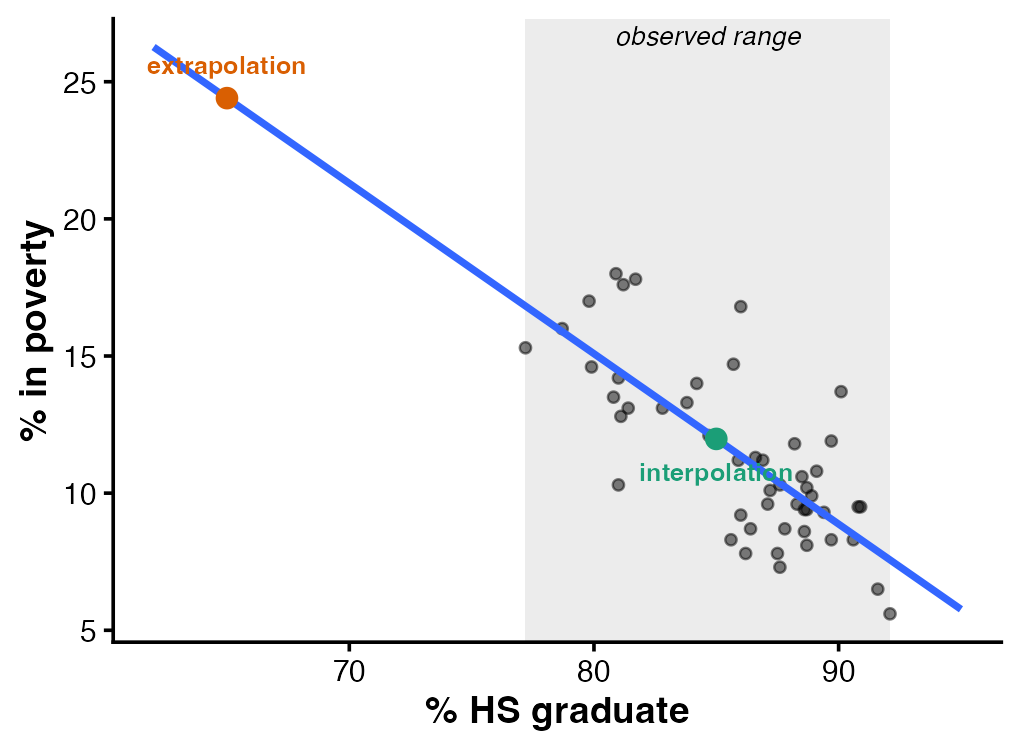
\includegraphics[width=\textwidth]{figures/extrapolation.png}
\end{center}
\end{column}
\end{columns}

\end{frame}
%%%%%%%%%%%%%%%%%%%%%%%%%%%%%%%%%%%%%%%%%%%%%%%%%%%%%%%%%%%%%%%%%%%%%%%%
\begin{frame}
\frametitle{Why extrapolation is risky}

\caution{Outside the observed range, the data give no support for the line: the pattern may not continue, and predictions can be nonsensical.}

\dq{A fitted model uses house sizes from $800$ to $3500$ square feet. How risky is the prediction for each of the following house sizes?\hspace{-1em}
\begin{itemize}
\item 700 square feet
\item $1{,}200$ square feet
\item $3{,}300$ square feet
\item $4{,}000$ square feet 
\end{itemize}}

\end{frame}
%%%%%%%%%%%%%%%%%%%%%%%%%%%%%%%%%%%%%%%%%%%%%%%%%%%%%%%%%%%%%%%%%%%%%%%%
\begin{frame}
\frametitle{Activity: prediction checklist}

\activity[-- using the fitted model]{%
For $\widehat{\text{poverty}}=64.78-0.62(\text{HS grad})$:
\begin{enumerate}
\item Predict poverty when the HS graduation rate is $90\%$.
\item If the observed poverty rate is $7.5\%$, compute the residual.
\item The data range from $77\%$ to $92\%$ --- is this prediction interpolation or extrapolation?
\end{enumerate}}

\pause
\solnbox{Prediction: $64.78-0.62(90)=8.98$. Residual: $7.5-8.98=-1.48$. Interpolation ($90\%$ lies within $77$--$92\%$).}

\end{frame}
%%%%%%%%%%%%%%%%%%%%%%%%%%%%%%%%%%%%%%%%%%%%%%%%%%%%%%%%%%%%%%%%%%%%%%%%
\section{Categorical predictors}
%%%%%%%%%%%%%%%%%%%%%%%%%%%%%%%%%%%%%%%%%%%%%%%%%%%%%%%%%%%%%%%%%%%%%%%%
\subsection{Indicator variables}
%%%%%%%%%%%%%%%%%%%%%%%%%%%%%%%%%%%%%%%%%%%%%%%%%%%%%%%%%%%%%%%%%%%%%%%%
\begin{frame}
\frametitle{Preview: a categorical predictor}

So far $x$ has been numerical. We can also use a \emph{category} by coding it as a $0/1$ \hl{indicator} (dummy) variable:
$$
\text{south}=\begin{cases}
1, & \text{Southern state},\\
0, & \text{otherwise}.
\end{cases}
$$
\keyidea[-- Indicator variable]{A $0/1$ indicator lets a regression use a categorical predictor. The category coded $0$ is the \hl{reference level}.}

\end{frame}
%%%%%%%%%%%%%%%%%%%%%%%%%%%%%%%%%%%%%%%%%%%%%%%%%%%%%%%%%%%%%%%%%%%%%%%%
\begin{frame}
\frametitle{Fitting poverty on region}

\begin{columns}[T]
\begin{column}{0.48\textwidth}
Fitted on the state data:
$$\widehat{\text{poverty}}=10.19+3.47(\text{south}).$$
{\small
Intercept $=$ \hl{reference-group mean} (Not South). Coefficient $=$ \hl{difference} in group means: $13.66-10.19=3.47$.}

\vspace{0.3em}
\textbf{Interpret $3.47$ in one sentence.}

\pause
\soln{Southern states are predicted to have poverty about $3.5$ points higher.}
\end{column}
\begin{column}{0.52\textwidth}
\begin{center}
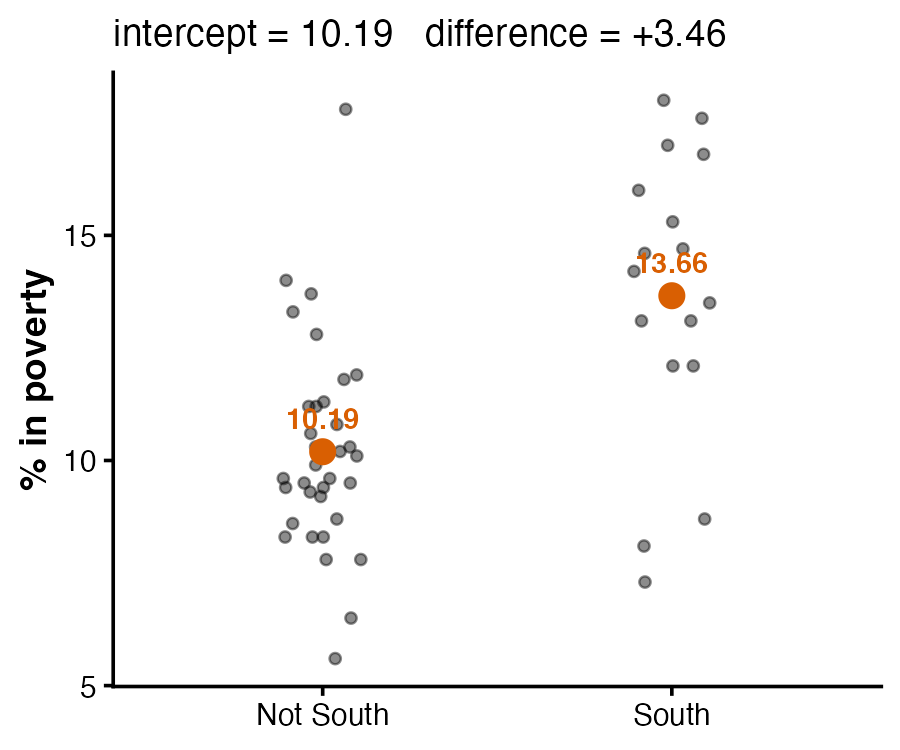
\includegraphics[width=0.86\textwidth]{figures/poverty-by-region.png}
\end{center}
\end{column}
\end{columns}

\end{frame}
%%%%%%%%%%%%%%%%%%%%%%%%%%%%%%%%%%%%%%%%%%%%%%%%%%%%%%%%%%%%%%%%%%%%%%%%
\begin{frame}
\frametitle{Practice: identify the reference level}

\activity[-- reference level]{A model reports coefficients for \texttt{region1} and \texttt{region2}, but none for \texttt{region3}. Which region is the reference level, and what does the intercept equal?}

\pause
\solnbox{\texttt{region3}: the reference category is the one omitted from the coefficient table, and the intercept is its predicted mean. In general, a $k$-level category needs $k-1$ indicators.}

\end{frame}
%%%%%%%%%%%%%%%%%%%%%%%%%%%%%%%%%%%%%%%%%%%%%%%%%%%%%%%%%%%%%%%%%%%%%%%%
\section{Wrap-up}
%%%%%%%%%%%%%%%%%%%%%%%%%%%%%%%%%%%%%%%%%%%%%%%%%%%%%%%%%%%%%%%%%%%%%%%%
\begin{frame}
\frametitle{Today's workflow}

\begin{enumerate}
\item \textbf{How strong?} Use $r$ for direction/strength and $R^2$ for the percent of variability explained.
\item \textbf{What prediction?} Substitute $x$ into the fitted equation; the residual $y-\widehat{y}$ is the prediction error.
\item \textbf{Is it reasonable?} Check whether $x$ is inside the observed range --- interpolation, not extrapolation.
\item \emph{Preview:} a $0/1$ indicator lets a categorical predictor into the model, with the omitted level as reference.
\end{enumerate}

\end{frame}
%%%%%%%%%%%%%%%%%%%%%%%%%%%%%%%%%%%%%%%%%%%%%%%%%%%%%%%%%%%%%%%%%%%%%%%%
\begin{frame}
\frametitle{Coming up next:}

Today: using a fitted line --- $r$ and $R^2$, prediction and extrapolation, and a first look at indicator variables.

\vspace{0.5em}
\hl{Next class --- Multiple regression:} what changes when a model uses \emph{several} predictors at once?

\begin{itemize}
\item the multiple regression model, and reading each coefficient \emph{holding the others fixed}
\item categorical predictors with more than two levels, through indicator variables
\item comparing models with $R^2$ and \hl{adjusted $R^2$}
\end{itemize}

\end{frame}
%%%%%%%%%%%%%%%%%%%%%%%%%%%%%%%%%%%%%%%%%%%%%%%%%%%%%%%%%%%%%%%%%%%%%%%%

%%%%%%%%%%%%%%%%%%%%%%%%%%%%%%%%%%%%
% End document
%%%%%%%%%%%%%%%%%%%%%%%%%%%%%%%%%%%%

\end{document}